\documentclass[10pt,a4paper]{article}

\usepackage[utf8]{inputenc}
\usepackage[T1]{fontenc}
\usepackage{geometry}
\geometry{a4paper, margin=1.4cm, top=1.4cm, bottom=1.4cm}

\usepackage{xcolor}
\definecolor{sapblue}{HTML}{0070D2}
\definecolor{sapdark}{HTML}{0B192C}
\definecolor{succgreen}{HTML}{059669}
\definecolor{alertred}{HTML}{DC2626}
\definecolor{warnamber}{HTML}{D97706}
\definecolor{softgray}{HTML}{F8FAFC}
\definecolor{bordergray}{HTML}{CBD5E1}

\usepackage{tikz}
\usetikzlibrary{shapes.geometric, arrows.meta, positioning, fit, backgrounds, calc}

\usepackage{booktabs}
\usepackage{array}
\usepackage{titlesec}
\usepackage{enumitem}
\usepackage{tcolorbox}
\usepackage{hyperref}

\hypersetup{
    colorlinks=true,
    linkcolor=sapblue,
    urlcolor=sapblue,
    pdftitle={Confronto Architetturale Workflow: Legacy vs SAP BTP},
    pdfauthor={Antigravity for Antonio}
}

% Compact titles
\titleformat{\section}
  {\normalfont\large\bfseries\color{sapdark}}{\thesection}{0.8em}{}[\vspace{-4pt}\color{sapblue}\titlerule]
\titleformat{\subsection}
  {\normalfont\normalsize\bfseries\color{sapblue}}{\thesubsection}{0.8em}{}

\titlespacing*{\section}{0pt}{8pt}{4pt}
\titlespacing*{\subsection}{0pt}{6pt}{2pt}
\setlist{itemsep=1.5pt, topsep=2pt, parsep=0pt}

\begin{document}

% Header Box
\begin{tcolorbox}[colback=sapblue!6!white, colframe=sapblue, title={\bfseries\large Confronto Architetturale dei Workflow: Legacy (SAP GUI) vs.\ SAP BTP}, fonttitle=\sffamily, top=4pt, bottom=4pt, left=8pt, right=8pt]
\sffamily\footnotesize
\textbf{Ambito Tecnico:} Evoluzione dal modello frammentato (SAP GUI + Excel + Email) alla piattaforma cloud enterprise integrata.\\
\textbf{Caso di Studio:} Rilevamento anomalie di prezzo fornitori, validazione e blocco tempestivo degli ordini di acquisto.
\end{tcolorbox}

\vspace{-4pt}

\section{Sintesi Comparativa dei Due Modelli}

\begin{table}[h!]
\centering
\footnotesize
\sffamily
\renewcommand{\arraystretch}{1.2}
\begin{tabular}{p{3.8cm} p{6.8cm} p{7.0cm}}
\toprule
\textbf{Parametro} & \textbf{Workflow Tradizionale (Legacy)} & \textbf{Workflow Moderno (SAP BTP)} \\
\midrule
\textbf{Interfaccia Utente} & SAP GUI client desktop anni '90, rigido e monolitico. & Web / Mobile responsive nativo (\textbf{SAP Fiori / Work Zone}). \\
\textbf{Tempo Preparazione} & 1 -- 3 ore di copia-incolla ed export manuale. & \textbf{0 secondi} (dati federati live in streaming in memoria). \\
\textbf{Analisi Anomalie} & Manuale con \texttt{CERCA.VERT} e Pivot su PC locale. & Assistita da AI e \textbf{Smart Assist} in \textbf{SAP Analytics Cloud}. \\
\textbf{Canale di Notifica} & Email manuale con file Excel allegato non protetto. & Notifica Push istantanea (MS Teams / Smartphone del manager). \\
\textbf{Esecuzione Azione} & Rientro manuale su SAP GUI (\texttt{ME22N}) per bloccare. & \textbf{Pulsante integrato} nella schermata Fiori $\rightarrow$ Event Mesh. \\
\textbf{Integrità ERP} & Rischio di personalizzazioni invasive (\textit{oggetti Z}). & \textbf{Clean Core}: ERP intatto, microservizi esterni via API OData. \\
\textbf{Sicurezza / GDPR} & Shadow IT: file riservati sparsi su desktop e mail. & Dati crittografati, token \textbf{OAuth 2.0 / IAS}, audit log completo. \\
\bottomrule
\end{tabular}
\end{table}

\vspace{-6pt}

\section{Il Vecchio Workflow (SAP GUI + Fogli Excel + Email)}

\begin{center}
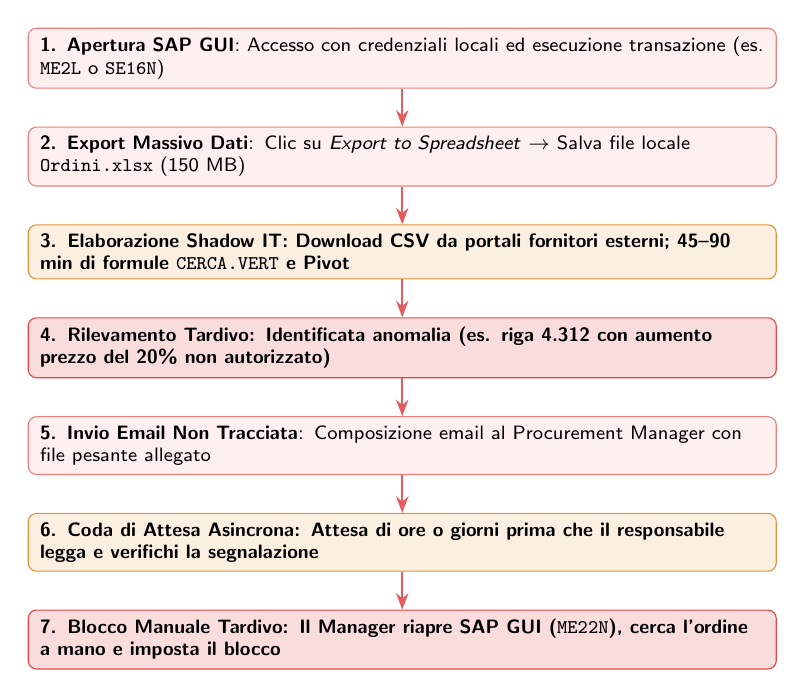
\begin{tikzpicture}[
  node distance=0.48cm and 0.8cm,
  boxStep/.style={
    rectangle, rounded corners=3pt, minimum width=9.5cm, minimum height=0.62cm,
    text width=9.2cm, align=left, fill=red!6, draw=alertred!60, font=\scriptsize\sffamily
  },
  boxAlert/.style={
    rectangle, rounded corners=3pt, minimum width=9.5cm, minimum height=0.62cm,
    text width=9.2cm, align=left, fill=warnamber!12, draw=warnamber!80, font=\scriptsize\bfseries\sffamily
  },
  boxCrit/.style={
    rectangle, rounded corners=3pt, minimum width=9.5cm, minimum height=0.62cm,
    text width=9.2cm, align=left, fill=alertred!16, draw=alertred!85, font=\scriptsize\bfseries\sffamily
  },
  arr/.style={-{Stealth[scale=0.9]}, thick, draw=alertred!75}
]

\node[boxStep] (step1) {\textbf{1. Apertura SAP GUI}: Accesso con credenziali locali ed esecuzione transazione (es. \texttt{ME2L} o \texttt{SE16N})};
\node[boxStep, below=of step1] (step2) {\textbf{2. Export Massivo Dati}: Clic su \textit{Export to Spreadsheet} $\rightarrow$ Salva file locale \texttt{Ordini.xlsx} (150 MB)};
\node[boxAlert, below=of step2] (step3) {\textbf{3. Elaborazione Shadow IT}: Download CSV da portali fornitori esterni; 45--90 min di formule \texttt{CERCA.VERT} e Pivot};
\node[boxCrit, below=of step3] (step4) {\textbf{4. Rilevamento Tardivo}: Identificata anomalia (es. riga 4.312 con aumento prezzo del 20\% non autorizzato)};
\node[boxStep, below=of step4] (step5) {\textbf{5. Invio Email Non Tracciata}: Composizione email al Procurement Manager con file pesante allegato};
\node[boxAlert, below=of step5] (step6) {\textbf{6. Coda di Attesa Asincrona}: Attesa di ore o giorni prima che il responsabile legga e verifichi la segnalazione};
\node[boxCrit, below=of step6] (step7) {\textbf{7. Blocco Manuale Tardivo}: Il Manager riapre SAP GUI (\texttt{ME22N}), cerca l'ordine a mano e imposta il blocco};

\draw[arr] (step1) -- (step2);
\draw[arr] (step2) -- (step3);
\draw[arr] (step3) -- (step4);
\draw[arr] (step4) -- (step5);
\draw[arr] (step5) -- (step6);
\draw[arr] (step6) -- (step7);

\end{tikzpicture}
\end{center}

\newpage

\section{Il Nuovo Workflow Moderno con SAP BTP}

Nel paradigma cloud-native di BTP, l'elaborazione \`e continua, reattiva agli eventi e integrata senza duplicare dati.

\vspace{0.2cm}

\begin{center}
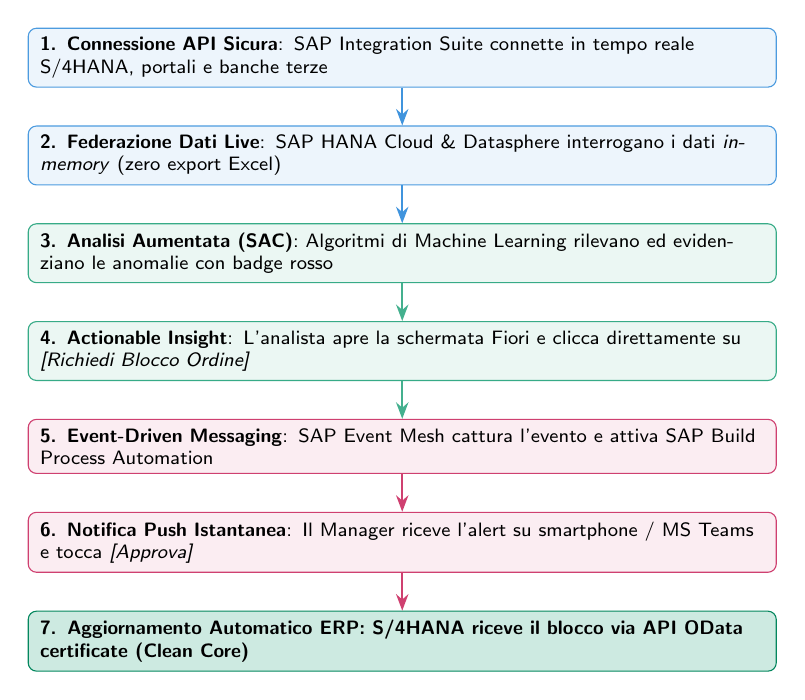
\begin{tikzpicture}[
  node distance=0.48cm and 0.8cm,
  boxData/.style={
    rectangle, rounded corners=3pt, minimum width=9.5cm, minimum height=0.62cm,
    text width=9.2cm, align=left, fill=sapblue!7, draw=sapblue!70, font=\scriptsize\sffamily
  },
  boxApp/.style={
    rectangle, rounded corners=3pt, minimum width=9.5cm, minimum height=0.62cm,
    text width=9.2cm, align=left, fill=succgreen!8, draw=succgreen!80, font=\scriptsize\sffamily
  },
  boxAuto/.style={
    rectangle, rounded corners=3pt, minimum width=9.5cm, minimum height=0.62cm,
    text width=9.2cm, align=left, fill=purple!7, draw=purple!75, font=\scriptsize\sffamily
  },
  boxFinal/.style={
    rectangle, rounded corners=3pt, minimum width=9.5cm, minimum height=0.62cm,
    text width=9.2cm, align=left, fill=succgreen!20, draw=succgreen!90!black, font=\scriptsize\bfseries\sffamily
  },
  arrBTP/.style={-{Stealth[scale=0.9]}, thick, draw=sapblue!75},
  arrApp/.style={-{Stealth[scale=0.9]}, thick, draw=succgreen!75},
  arrAuto/.style={-{Stealth[scale=0.9]}, thick, draw=purple!75}
]

\node[boxData] (b1) {\textbf{1. Connessione API Sicura}: SAP Integration Suite connette in tempo reale S/4HANA, portali e banche terze};
\node[boxData, below=of b1] (b2) {\textbf{2. Federazione Dati Live}: SAP HANA Cloud \& Datasphere interrogano i dati \textit{in-memory} (zero export Excel)};
\node[boxApp, below=of b2] (b3) {\textbf{3. Analisi Aumentata (SAC)}: Algoritmi di Machine Learning rilevano ed evidenziano le anomalie con badge rosso};
\node[boxApp, below=of b3] (b4) {\textbf{4. Actionable Insight}: L'analista apre la schermata Fiori e clicca direttamente su \textit{[Richiedi Blocco Ordine]}};
\node[boxAuto, below=of b4] (b5) {\textbf{5. Event-Driven Messaging}: SAP Event Mesh cattura l'evento e attiva SAP Build Process Automation};
\node[boxAuto, below=of b5] (b6) {\textbf{6. Notifica Push Istantanea}: Il Manager riceve l'alert su smartphone / MS Teams e tocca \textit{[Approva]}};
\node[boxFinal, below=of b6] (b7) {\textbf{7. Aggiornamento Automatico ERP}: S/4HANA riceve il blocco via API OData certificate (\textit{Clean Core})};

\draw[arrBTP] (b1) -- (b2);
\draw[arrBTP] (b2) -- (b3);
\draw[arrApp] (b3) -- (b4);
\draw[arrApp] (b4) -- (b5);
\draw[arrAuto] (b5) -- (b6);
\draw[arrAuto] (b6) -- (b7);

\end{tikzpicture}
\end{center}

\vspace{-4pt}

\section{I 3 Pilastri Architetturali Fondamentali}

\begin{enumerate}[leftmargin=*]
    \item \textbf{Data Virtualization (Zero Copie)}: Con SAP HANA Cloud e Datasphere i dati non vengono duplicati o scaricati su supporti locali. Rimangono custoditi nel database centrale e vengono interrogati in tempo reale alla velocit\`a della RAM.
    \item \textbf{Actionable Insights (Dall'Analisi all'Azione)}: L'applicazione analitica cessa di essere un cruscotto passivo. L'interfaccia Fiori incorpora i pulsanti operativi per scatenare i processi transazionali all'istante.
    \item \textbf{Strategia Clean Core (Disaccoppiamento)}: Nessun programma personalizzato viene iniettato nel core dell'ERP S/4HANA. L'intera logica risiede su BTP e comunica via API standard, azzerando i costi di aggiornamento di versione.
\end{enumerate}

\vspace{0.1cm}

\begin{tcolorbox}[colback=softgray, colframe=bordergray, title={\sffamily\scriptsize\bfseries Cheat Sheet per Colloqui di Lavoro e Riunioni Tecniche}, top=3pt, bottom=3pt, left=6pt, right=6pt]
\sffamily\scriptsize
\begin{itemize}[leftmargin=10pt]
    \item \textbf{Perch\'e BTP genera ROI?} Elimina centinaia di ore/uomo perse in compiti manuali e blocca le perdite prima che le fatture vengano saldate.
    \item \textbf{Come garantisce la sicurezza?} Sostituisce la \textit{Shadow IT} con autenticazione federata OAuth 2.0 / OIDC gestita da SAP Cloud Identity Services.
    \item \textbf{Cos'\`e il Clean Core?} \`E la disciplina architetturale che preserva lo standard S/4HANA, delegando tutte le estensioni a microservizi \textit{side-by-side} su BTP.
\end{itemize}
\end{tcolorbox}

\end{document}
